% !TEX root = ../main_final.tex

\noind Nos exemples s'articulent autour du d�sassemblage du programme \ref{prog_original} qui a �t� obfusqu� en modifiant son graphe de flow (programme \ref{prog_obf_cfg}) et en ind�terminant ses branches (programme \ref{prog_obf_saut_cond})

%% !TEX root = ../main.tex

\begin{lstlisting}[caption=\texttt{fibo} en assembleur, label=fiboasm, keywordstyle=\color{black}]
start:
0000000100000e20	pushq	$0x00
0000000100000e22	movq	%rsp,%rbp
0000000100000e25	andq	$0xf0,%rsp
0000000100000e29	movq	0x08(%rbp),%rdi
0000000100000e2d	leaq	0x10(%rbp),%rsi
0000000100000e31	movl	%edi,%edx
0000000100000e33	addl	$0x01,%edx
0000000100000e36	shll	$0x03,%edx
0000000100000e39	addq	%rsi,%rdx
0000000100000e3c	movq	%rdx,%rcx
0000000100000e3f	jmp	0x100000e45
0000000100000e41	addq	$0x08,%rcx
0000000100000e45	cmpq	$0x00,(%rcx)
0000000100000e49	jne	0x100000e41
0000000100000e4b	addq	$0x08,%rcx
0000000100000e4f	callq	_main
0000000100000e54	movl	%eax,%edi
0000000100000e56	callq	0x100000f02	; stub for: _exit
0000000100000e5b	hlt
0000000100000e5c	nop
0000000100000e5d	nop
0000000100000e5e	nop
0000000100000e5f	nop
_fibo:
0000000100000e60	pushq	%rbp
0000000100000e61	movq	%rsp,%rbp
0000000100000e64	subq	$0x10,%rsp
0000000100000e68	movl	%edi,0xfc(%rbp)
0000000100000e6b	movl	0xfc(%rbp),%eax
0000000100000e6e	cmpl	$0x00,%eax
0000000100000e71	jne	0x100000e7c
0000000100000e73	movl	$0x00000001,0xf4(%rbp)
0000000100000e7a	jmp	0x100000eb6
0000000100000e7c	movl	0xfc(%rbp),%eax
0000000100000e7f	cmpl	$0x01,%eax
0000000100000e82	jne	0x100000e8d
0000000100000e84	movl	$0x00000001,0xf4(%rbp)
0000000100000e8b	jmp	0x100000eb6
0000000100000e8d	movl	0xfc(%rbp),%eax
0000000100000e90	subl	$0x01,%eax
0000000100000e93	movl	%eax,%edi
0000000100000e95	callq	_fibo
0000000100000e9a	movl	%eax,%ecx
0000000100000e9c	movl	0xfc(%rbp),%edx
0000000100000e9f	subl	$0x02,%edx
0000000100000ea2	movl	%edx,%edi
0000000100000ea4	movl	%ecx,0xf0(%rbp)
0000000100000ea7	callq	_fibo
0000000100000eac	movl	%eax,%ecx
0000000100000eae	movl	0xf0(%rbp),%edx
0000000100000eb1	addl	%ecx,%edx
0000000100000eb3	movl	%edx,0xf4(%rbp)
0000000100000eb6	movl	0xf4(%rbp),%eax
0000000100000eb9	movl	%eax,0xf8(%rbp)
0000000100000ebc	movl	0xf8(%rbp),%eax
0000000100000ebf	addq	$0x10,%rsp
0000000100000ec3	popq	%rbp
0000000100000ec4	ret
0000000100000ec5	nopl	0x00(%rax,%rax)
0000000100000eca	nopw	0x00(%rax,%rax)
_main:
0000000100000ed0	pushq	%rbp
0000000100000ed1	movq	%rsp,%rbp
0000000100000ed4	subq	$0x10,%rsp
0000000100000ed8	movl	$0x00000005,%eax
0000000100000edd	movl	%eax,%edi
0000000100000edf	callq	_fibo
0000000100000ee4	movl	%eax,%ecx
0000000100000ee6	xorb	%dl,%dl
0000000100000ee8	leaq	0x00000045(%rip),%rdi
0000000100000eef	movl	%ecx,%esi
0000000100000ef1	movb	%dl,%al
0000000100000ef3	callq	0x100000f08; stub for: _printf
0000000100000ef8	movl	0xfc(%rbp),%eax
0000000100000efb	addq	$0x10,%rsp
0000000100000eff	popq	%rbp
0000000100000f00	ret
\end{lstlisting}


\begin{lstlisting}[caption=Programme non obfusqu�,  language={[x86masm]Assembler}, label=prog_original]
main:
	mov eax, 3
	mov ebx, 36
	add eax, ebx
	imul ecx, ebx, 2
	sub eax, ebx
	hlt
\end{lstlisting}

\begin{lstlisting}[caption=Obfuscation par modification du graphe de flow,  language={[x86masm]Assembler}, label=prog_obf_cfg]
main:
	mov eax, 3
	jmp a    
b:
	add eax, ebx
	jmp c
e:
	mov eax, ecx
	and esp, ebp
d:
	sub eax, ebx
	hlt
a:
	mov ebx, 36
	jmp b
c:
	imul ecx, ebx, 2
	jmp d
\end{lstlisting}


\begin{lstlisting}[caption=Obfuscation par ind�termination des branches,  language={[x86masm]Assembler}, label=prog_obf_saut_cond]
main:
	mov eax, 3
	cmp eax, 3
	je a
b:
	add eax, ebx
	cmp eax, 39
	je c
e:
	mov eax, ecx
	and esp, ebp
d:
	sub eax, ebx
	cmp eax, 3
	jne e
	hlt
a:
	mov ebx, 36
	cmp ebx, 36
	je b
c:
	imul ecx, ebx, 2
	cmp ecx, 72
	je d
\end{lstlisting}

%\begin{figure}[p]
%\centering
%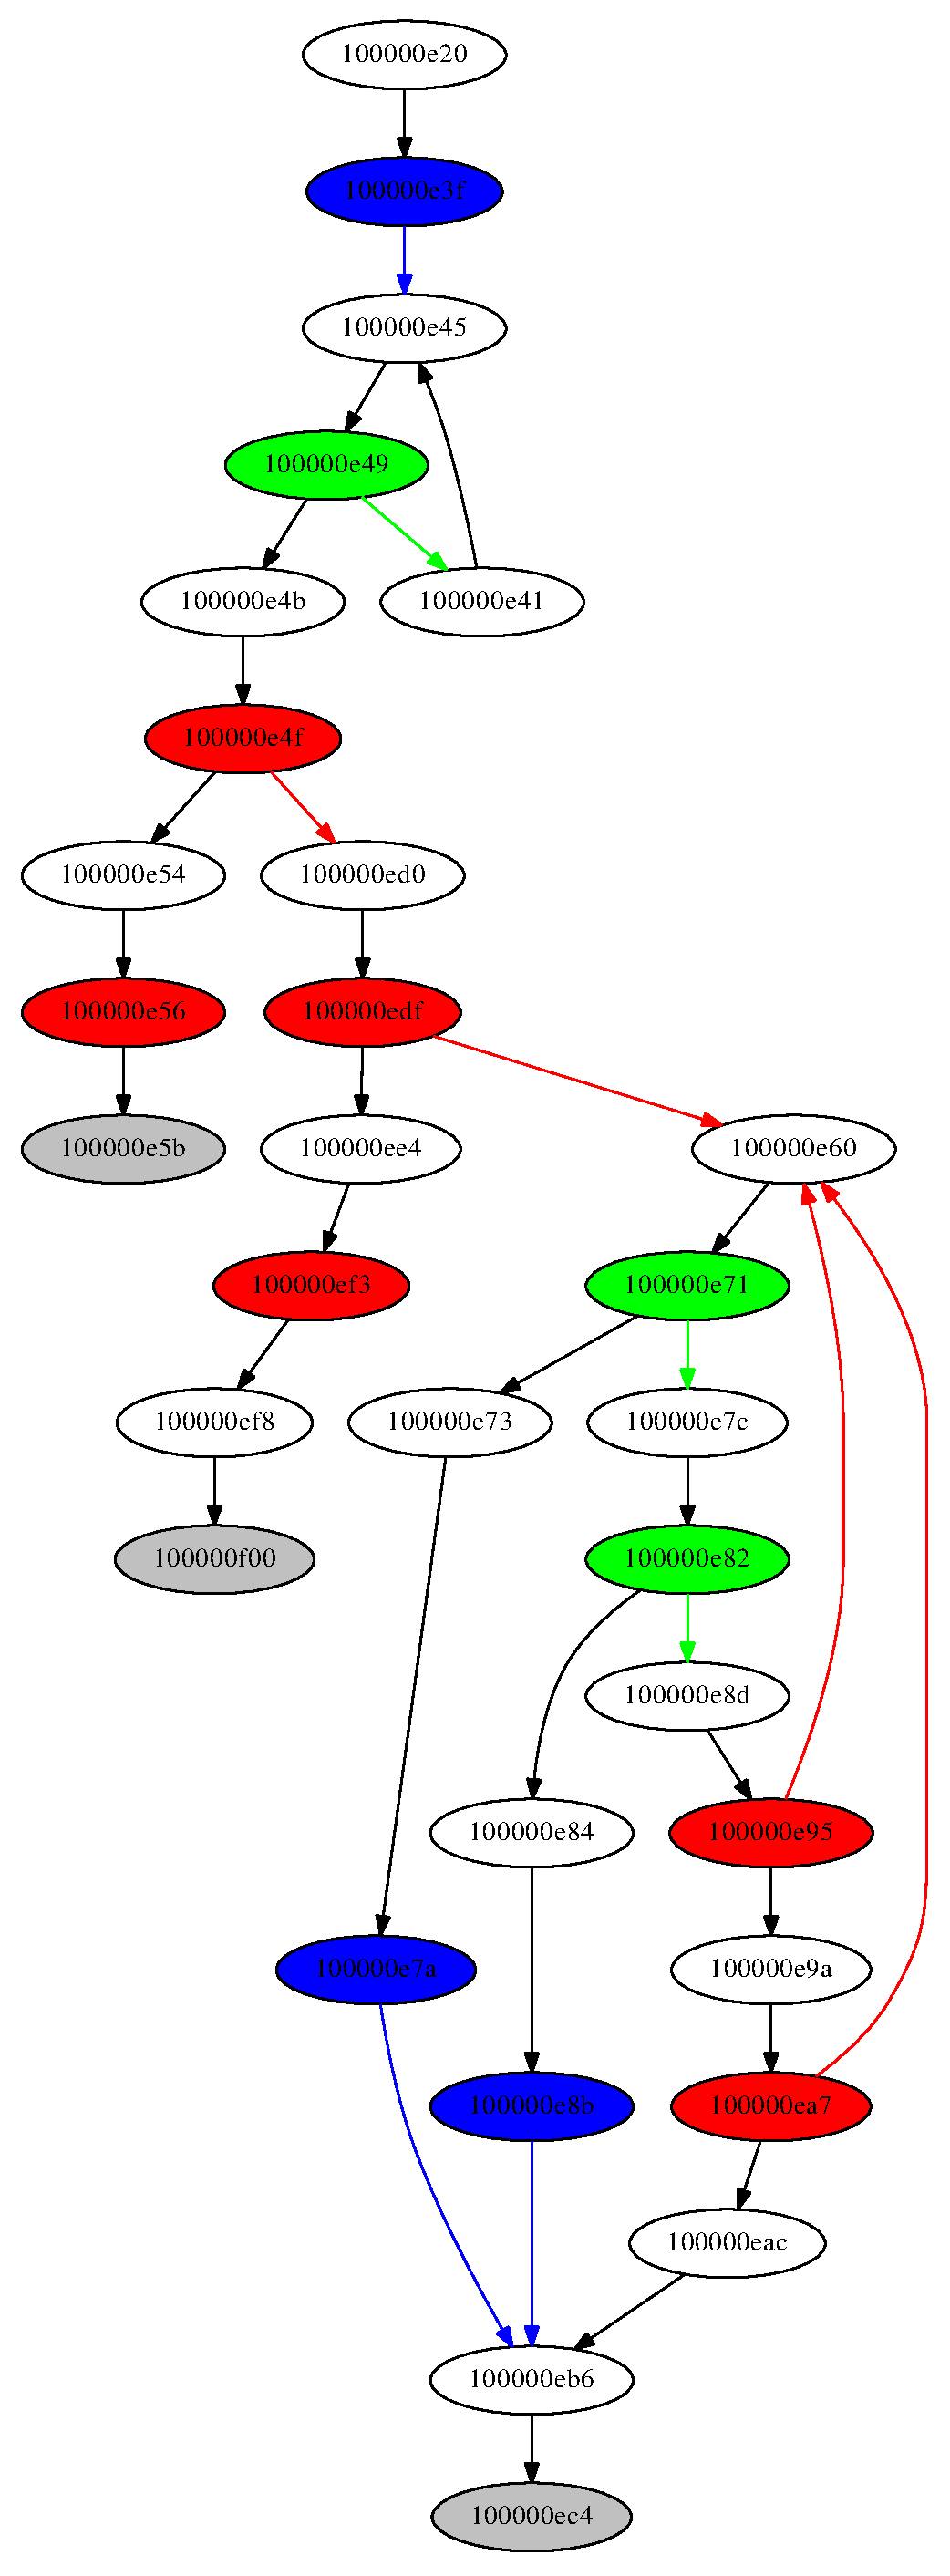
\includegraphics[width=7.4cm]{input/recc.eps}
%\caption{Graphe de flow de \texttt{fibo}}
%\label{CFGfibo}
%\end{figure}